\section{Recycling Robots}

Come si può intuire dal nome, la scena contiene dei robot, i quali hanno il compito di riciclare la spazzatura presente nell'ambiente portandola nel rispettivo bidone. Il compito generale di un robot è divisibile in un ciclo di sotto-obiettivi, ad esempio:
\begin{enumerate}
    \item Cercare la spazzatura;
    \item Andare verso la spazzatura trovata;
    \item Prendere la spazzatura appena raggiunta;
    \item Cercare il bidone;
    \item Andare verso il bidone trovato;
    \item Riciclare la spazzatura.
\end{enumerate}

In questo particolare scenario è stato deciso di simulare la presenza di diversi tipi di spazzatura (plastica, vetro e carta) e, di conseguenza, sono stati creati diversi tipi di robot e bidoni.

\begin{figure}[H]
\centering
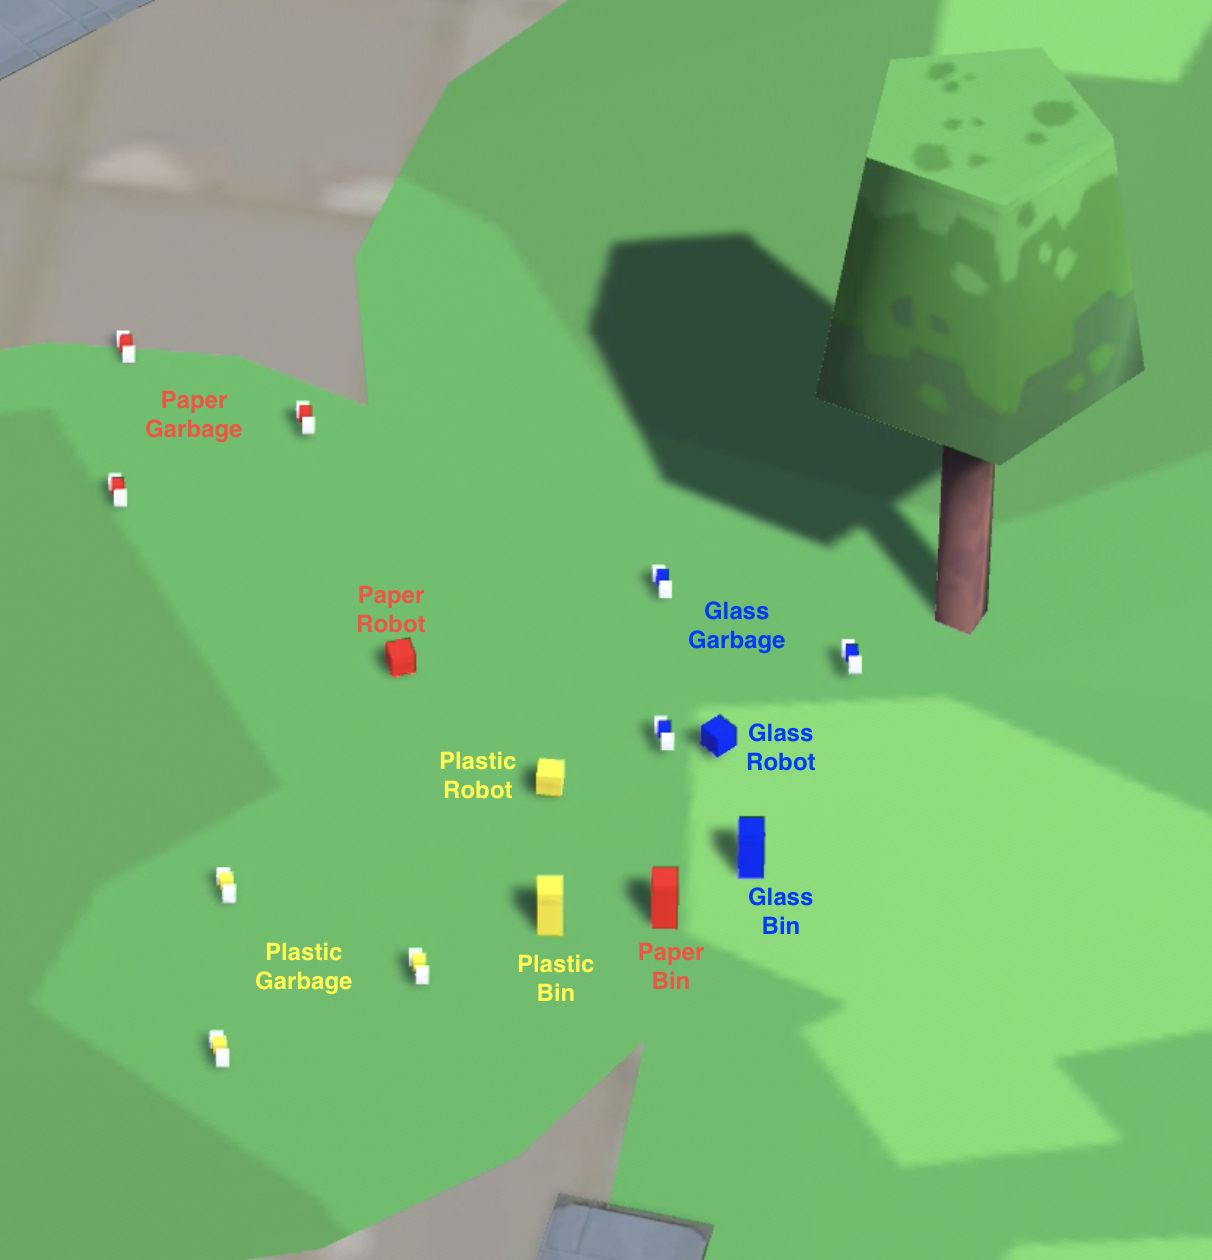
\includegraphics[width=\textwidth]{figures/recycling_robots.png}
\caption{Scenario Recycling Robots}
\label{scenario_recycling_robots}
\end{figure}

Ogni oggetto in scena è stato considerato come entità, con l'unica differenza che solo i robot sono dotati di autonomia attraverso un agente JASON ad essi collegato. La spazzatura ed i bidoni sono entità che, lato MAS, si fermano al concetto di artefatto. Per realizzare la scena è stato utilizzato WRLD \cite{wrld} che fornisce mappe 3D costruite usando dati geografici di alta qualità da poter utilizzare per la creazione di visualizzazioni 3D, esecuzione di simulazioni, o per lo sviluppo di giochi o esperienze dinamiche, basati sulla posizione geografica.

\subsection{Robot}

In questa sezione sono presenti i listati realizzati per definire il corpo e la mente dell'entità Robot.

\subsubsection{Corpo}

\lstinputlisting[label={robot},caption={Robot},language={[Sharp]C}]{code/Robot.cs}

Come da listato \ref{robot}, è stato realizzato uno script \textit{Robot}, che estende \textit{SynapsisBody}, il quale viene collegato al GameObject che rappresenta il robot nella scena Unity.
La presenza di API predefinite, all'interno di \textit{SynapsisBody}, ha ampiamente coperto tutte le attività che il robot deve svolgere in questo particolare scenario, difatti l'unica azione da definire è stata la colorazione del robot in base alla tipologia di spazzatura che è in grado di riciclare.

\subsubsection{Mente}

\lstinputlisting[label={robotArtifact},caption={Artefatto del robot},language={Java}]{code/RobotMind.java}

Il listato \ref{robotArtifact} definisce l'artefatto utilizzato nel MAS per collegarsi al middleware. Estendendo la classe \textit{SynapsisMind} è stato necessario definire una sola azione specifica che riguarda la colorazione del corpo del robot in base alla tipologia di spazzatura che lui è in grado di riciclare. 

\lstinputlisting[label={robotAgent},caption={Agente del robot},language={asl}]{code/robot.asl}

Il listato \ref{robotAgent} rappresenta l'agente JASON realizzato per definire l'automazione del robot. I beliefs iniziali sono utilizzati per definire il collegamento al middleware, mente il goal iniziale serve ad istanziare l'artefatto realizzato dell'immagine precedente \ref{robotArtifact}.

\medskip

Il plan \textit{synapsis\_counterpart\_status(Name, C)} è stato utilizzato per avviare l'obiettivo di "riciclare" del robot, mentre i successivi piani (\textit{stopped},\textit{found(Name)},\textit{arrived\_to(Name)}, \textit{picked(Name)}, \textit{released(Name)}) sono stati definiti per reagire alle percezioni inviabili dal corpo. I piani che iniziano per \textit{recycle} rappresentano tutte le fasi che il robot può utilizzare per riciclare la spazzatura.

\medskip

Nella parte finale del listato si può vedere in che modo è stata effettuata l'importazione dell'agente base presente nella libreria per JaCaMo.

\subsection{Bidone}

In questa sezione sono presenti i listati realizzati per definire il corpo e l'artefatto dell'entità Bidone.

\subsubsection{Corpo}

\lstinputlisting[label={bidone},caption={Script per il corpo del bidone},language={[Sharp]C}]{code/Bin.cs}

Come da listato \ref{bidone}, è stato realizzato un script \textit{Bin}, che estende \textit{SynapsisBody}, il quale viene collegato al GameObject che rappresenta il bidone nella scena Unity. L'unica azione da definire è stata la colorazione del GameObject "bidone" in base alla tipologia di spazzatura da lui accettata.

\subsubsection{Mente}

\lstinputlisting[label={binArtifact},caption={Artefatto del bidone},language={Java}]{code/BinMind.java}

Il listato \ref{binArtifact} definisce l'artefatto utilizzato nel MAS per collegarsi al middleware. Estendendo la classe \textit{SynapsisMind} è stato necessario definire una sola azione specifica che riguarda la colorazione del corpo del bidone in base alla tipologia di spazzatura da lui accettata. 

\subsection{Spazzatura}

In questa sezione sono presenti i listati realizzati per definire il corpo e l'artefatto dell'entità Spazzatura.

\subsubsection{Corpo}

\lstinputlisting[label={spazzatura},caption={Script per il corpo della spazzatura},language={[Sharp]C}]{code/Garbage.cs}

Come da listato \ref{spazzatura}, è stato realizzato uno script \textit{Garbage}, che estende \textit{SynapsisBody}, il quale viene collegato al GameObject che rappresenta la spazzatura nella scena Unity. Le azione da definire sono state la colorazione del GameObject "spazzatura" in base alla tipologia di spazzatura rappresentata e l'azione \textit{recycle\_me} per disattivare (riciclare) il GameObject dalla scena.

\medskip

Il metodo \textit{OnTransformParentChanged} viene utilizzato per sapere quando la spazzatura viene raccolta da un robot cosi da inviare la percezione \textit{picked\_up\_by} alla mente. Questa percezione viene utilizzata dal robot per capire quando è entrato in possesso della spazzatura che ha raggiunto.

\subsubsection{Mente}

\lstinputlisting[label={garbageArtifact},caption={Artefatto della spazzatura},language={Java}]{code/GarbageMind.java}

Il listato \ref{garbageArtifact} definisce l'artefatto utilizzato nel MAS per collegarsi al middleware. Estendendo la classe \textit{SynapsisMind} è stato necessario definire due azioni specifiche: la prima riguarda la colorazione del corpo della spazzatura in base alla tipologia di spazzatura rappresentata; mentre la seconda permette di riciclare sè stessa. L'ultima azione viene utilizzata dal robot dopo aver portato la spazzatura nel bidone corretto.

\subsection{Esempio interazione}

Viene ora illustrata l'interazione tra corpo e mente dell'entità robot durante la ricerca del bidone.

\begin{figure}[H]
\centering
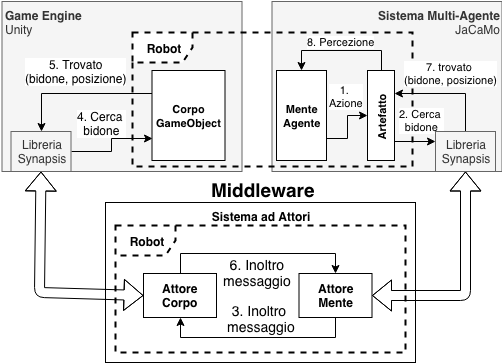
\includegraphics[width=\textwidth]{figures/scenario_esempio.png}
\caption{Esempio di comunicazione tra mente e corpo}
\label{scenario_esempio}
\end{figure}

L'immagine \ref{scenario_esempio} mostra il flusso ordinato di interazioni per l'esempio appena descritto. La mente per svolgere il plan \textit{"Cercare il bidone"} vuole inviare al proprio corpo l'azione \textit{"Cerca bidone"}. La richiesta di svolgere l'azione inizia dall'utilizzo dell'operazione presente nell'artefatto personale dell'agente\footnote{previa associazione dei due}, in possesso del canale per comunicare con il middleware.

\medskip

L'artefatto, quindi, invia il messaggio al middleware. L’attore "mente", presente nel middleware alla ricezione delle informazioni, inoltra le stesse all'attore "corpo", unico possessore del riferimento all’entità "corpo" presente su Unity in grado di inoltrare il messaggio al corpo "reale".  

\medskip

Alla ricezione del messaggio, l'entità corpo (GameObject) attua l'azione richiesta e risponde alla mente (Agente) inviandogli la percezione generata, ad esempio \textit{"trovato(nomeBidone)"}.

\medskip

A questo punto, la percezione viene mandata all'attore "corpo" nel middleware che, a sua volta, la inoltrerà all'attore "mente" e, di conseguenza, all'artefatto collegato. L'artefatto, nel momento in cui riceve la percezione, aggiunge quest'ultima alle sue proprietà osservabili che, automaticamente, aggiorneranno la BeliefBase dell'agente. 

\medskip

L'ultimo passaggio rappresenta il punto cruciale per completare il collegamento tra corpo e mente, dato che in questa maniera l'agente ha ricevuto la percezione dal proprio corpo. 

\subsubsection{Video dello scenario}

\'E possibile visualizzare lo scenario realizzato attraverso il video presente nel repository del middleware \ref{materiale_online}.